\section*{Chapter 2}


\exercise{2.1.1.2}
$\mathcal{P}(A) = \emptyset, \{1\}, \{2\}, \{3\}, \{1,2\}, \{1,3\}, \{2,3\}, \{1,2,3\}$


\exercise{2.1.1.3}
\paragraph{a.}
A function $PR \to RG$.
\paragraph{b.}
Yes, there are probably many many-to-one connection points.


\exercise{2.1.2.5}
\paragraph{a.}
$2 \mapsto 4$
\paragraph{b.}
$0 \mapsto 0$
\paragraph{c.}
Not applicable; $-2 \not\in \mathbb{N}$.
\paragraph{d.}
$5 \mapsto 25$
\paragraph{e.}
The symbol $\to$ associates the domain and codomain, while $\mapsto$
associates a particular member of the domain to a particular member of
the codomain.


\exercise{2.1.2.6}
$\operatorname{im}(f) = \{y_1, y_2, y_4\}$


\exercise{2.1.2.8}
$f(A) = \{0,1,4,9\}$


\exercise{2.1.2.10}
$f \circ x \colon \{\smiley\} \to Y$ and $\smiley \mapsto f(x)$.


\exercise{2.1.2.12}
\paragraph{a.}
$2^5 = 32$
\paragraph{b.}
$5^2 = 25$


\exercise{2.1.2.13}
\paragraph{a.}
Take $A := \{\smiley\}$.  (e.g. $A := $
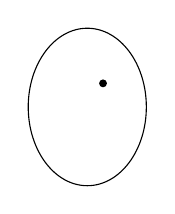
\begin{tikzpicture}
  \draw (0,0) ellipse [x radius = 0.75, y radius = 1];
  \fill (0.2,0.3) circle [radius=0.05] node[anchor=south]{\smiley};
\end{tikzpicture}
, $X := $
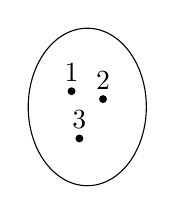
\begin{tikzpicture}
  \draw (0,0) ellipse [x radius = 0.75, y radius = 1];
  \fill (-0.2,0.2) circle [radius=0.05] node[anchor=south]{1};
  \fill (0.2,0.1) circle [radius=0.05] node[anchor=south]{2};
  \fill (-0.1,-0.4) circle [radius=0.05] node[anchor=south]{3};
\end{tikzpicture}
)
\paragraph{b.}
$B := \emptyset$.  (e.g. $B := $
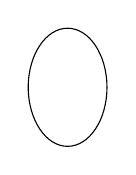
\begin{tikzpicture}
    \draw (0,0) ellipse [x radius = 0.50, y radius = 0.75];
\end{tikzpicture}
)


\exercise{2.1.2.17}
\paragraph{a.}
$n!\,$
\paragraph{b.}
Yes, $0! = 1$.


\exercise{2.1.2.19}
No.


\exercise{2.1.2.20}
Take $A := \{\smiley\}$.


\exercise{2.1.2.22}
\paragraph{a.}
$f(4) = c$
\paragraph{b.}
$f = \left(1,4,9,16,25,36,49\right)$


\exercise{2.1.2.24}
\paragraph{a.}
3
\paragraph{b.}
4
\paragraph{c.}
$\lvert\mathbb{N}\rvert \geqslant \infty$
\paragraph{d.}
$\lvert\lbrace n \in \mathbb{N} \mid n \leqslant 5 \rbrace \rvert =
 \lvert\lbrace 0,1,2,3,4,5\rbrace\rvert = 6$


\exercise{2.3.2.7}
\begin{tikzpicture}[->,>=stealth,shorten >=10pt,shorten <=10pt,auto]
  \node [shape=rectangle,draw,text width=4cm] (R)
  {
    a pair $(p,c)$, where $p$ is a person, $c$ is a child, and $p$ has
    $c$ as a child
  };
  \node [shape=rectangle,draw,below left=of R] (P) {a person};
  \node [shape=rectangle,draw,below right=of R] (C) {a child};

  \path (R) edge node {p} (P)
            edge node {c} (C);
\end{tikzpicture}


%%% Local Variables:
%%% mode: latex
%%% TeX-master: "exercises"
%%% End:
